\begin{solution}

\begin{enumerate}
\item We compute
  \begin{eqnarray*}
     {\d u\over \d t} &=& -\kappa \theta^2/(\rho c) e^{-\kappa \theta^2 t/(\rho c)} \sin(\theta x) \\[0.5em]
     {\d u\over \d x} &=& \theta e^{-\kappa \theta^2 t/(\rho c)} \cos(\theta x) \\[0.5em]
     {\d^2 u\over \d x^2} &=& -\theta^2 e^{-\kappa \theta^2 t/(\rho c)} \sin(\theta x).
  \end{eqnarray*}
With these formulas in hand it is easy to verify that 
 \[  \rho c {\d u \over \d t} = \kappa {\d^2 u\over \d x^2}.\]

\item We wish to find the values of $\theta$ that give homogeneous Dirichlet boundary conditions,
      i.e., $u(0,t) = u(\ell,t)=0$ for all $t$.
      Since $e^{-\kappa \theta^2 t/(\rho c)}$ is positive for all $t$, we can only get
      the homogeneous Dirichlet conditions when $\sin(\theta x)=0$.
      For any $\theta$, $\sin(\theta\cdot 0) = 0$, so the condition at $x=0$ is automatically
      satisfied.  To get $\sin(\theta \ell) = 0$, we need $\theta \ell$ 
      to be an integer multiple of $\pi$, that is,
           \[ \theta \ell = \pi n, \qquad n = 0, \pm 1, \pm 2, \ldots,\]
      or equivalently
           \[ \theta  = {\pi n\over \ell}, \qquad n = 0, \pm 1, \pm 2, \ldots.\]
      (Notice that if $n=0$ we have the trivial solution $u(x,t) =0 $ for all $x,t$.
       If $n=1$, we have a solution for which $u(x,t) \ge 0$ for all $x,t$.
       For other values of $n$ the solution will be \emph{negative} for some $x, t$.
       If our temperature is measured in Kelvin this could be a problem!
       However, this heat equation takes the same form if we shift to Celsius units,
       so we needn't be so troubled by the negative values of temperature.)

\item Since $n=0$ is trivial, we shall take $n=1$ ($\theta = \pi/\ell$) to obtain       
                  \begin{eqnarray*}
                        u(x,t) &=& e^{-\kappa \pi^2 t/(\ell^2 \rho c)} \sin(\pi x/\ell)  \\[0.5em]
                               &=& e^{-3.86 \pi^2 t/(100\cdot 8.96\cdot 0.385)} \sin(\pi x/10).
                  \end{eqnarray*}

\item Solutions are shown in the attached plots.  Any of these style is acceptable. 
      The MATLAB code that generated these plots follows. 

      [\textbf{GRADERS}: please make a note if students did not include their MATLAB code,
       but do not take off points for this first time.  You should do so in the future, though!]
        
      \begin{center}
           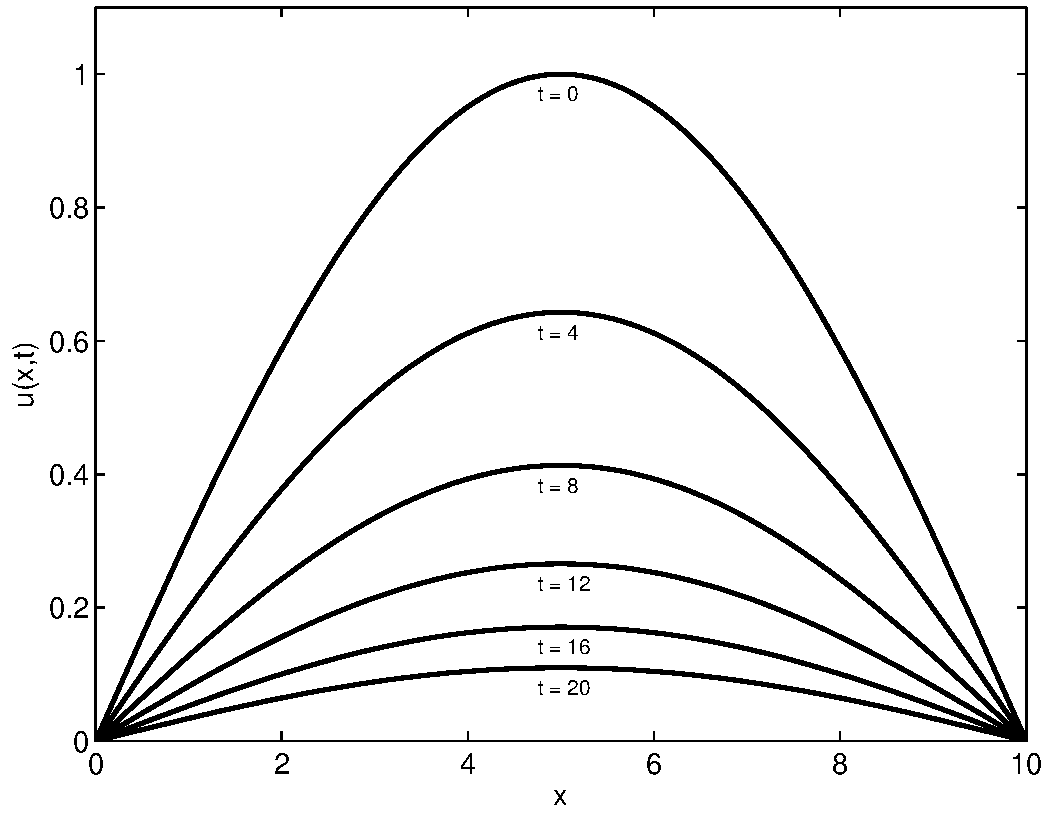
\includegraphics[scale=0.53]{checksol1}

           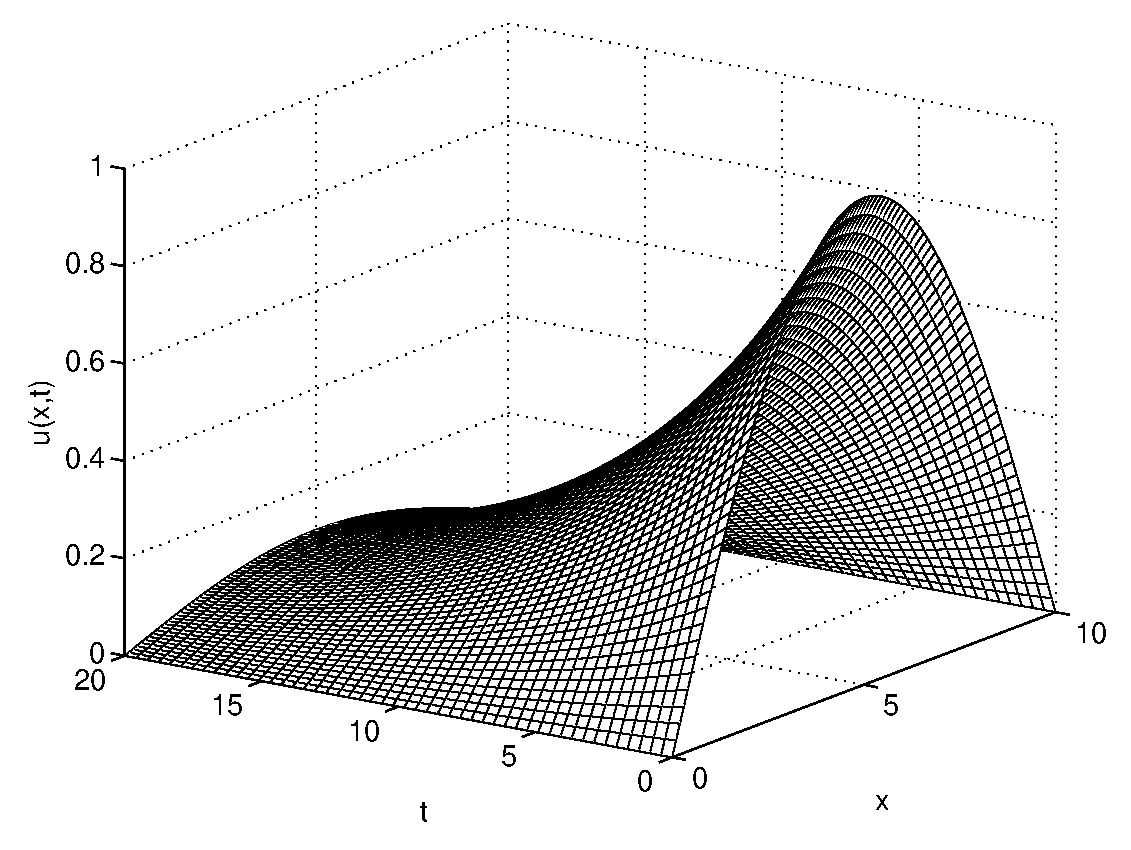
\includegraphics[scale=0.53]{checksol2}

           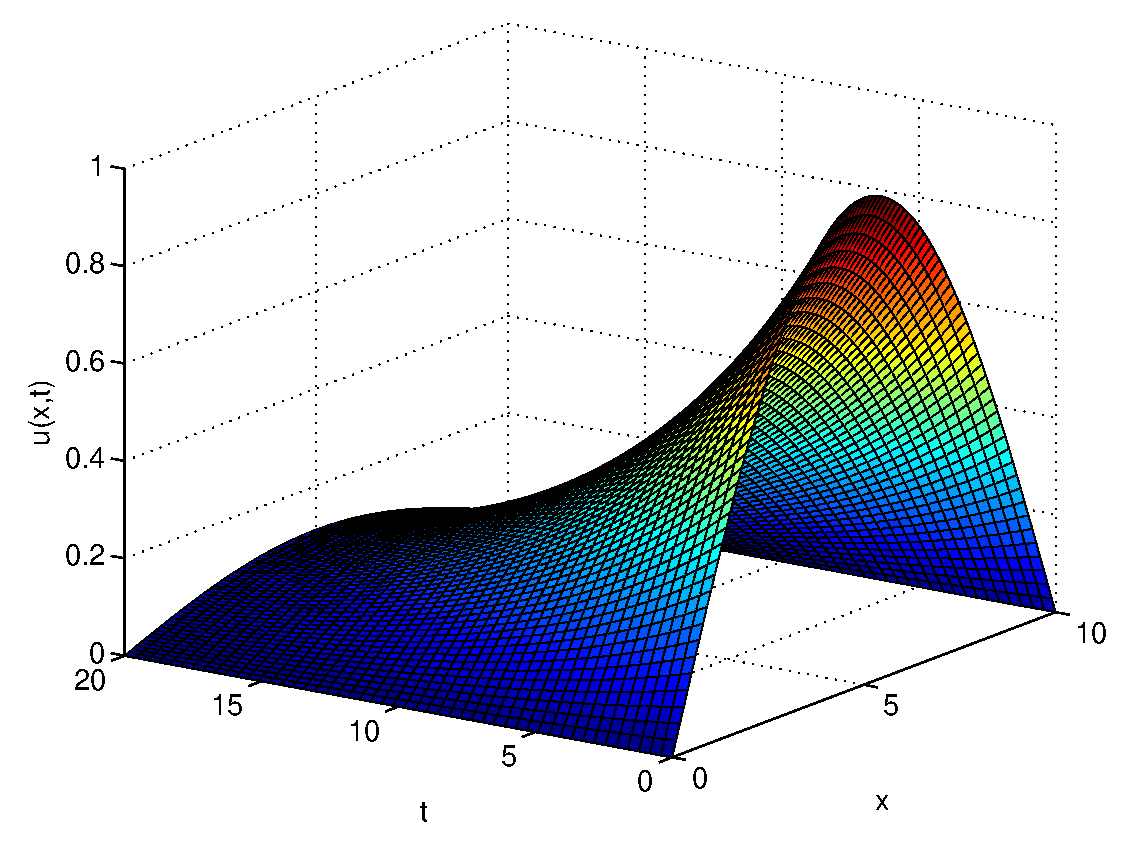
\includegraphics[scale=0.53]{checksol3}

           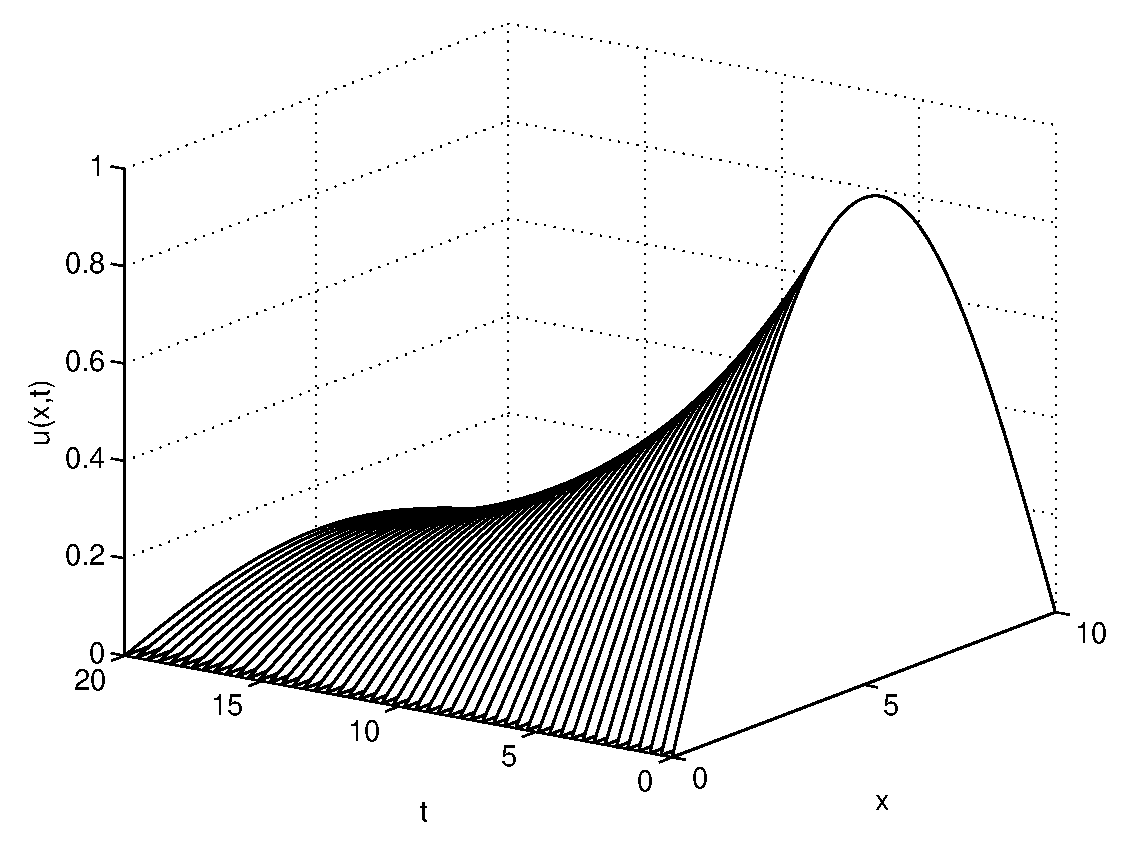
\includegraphics[scale=0.53]{checksol4}

           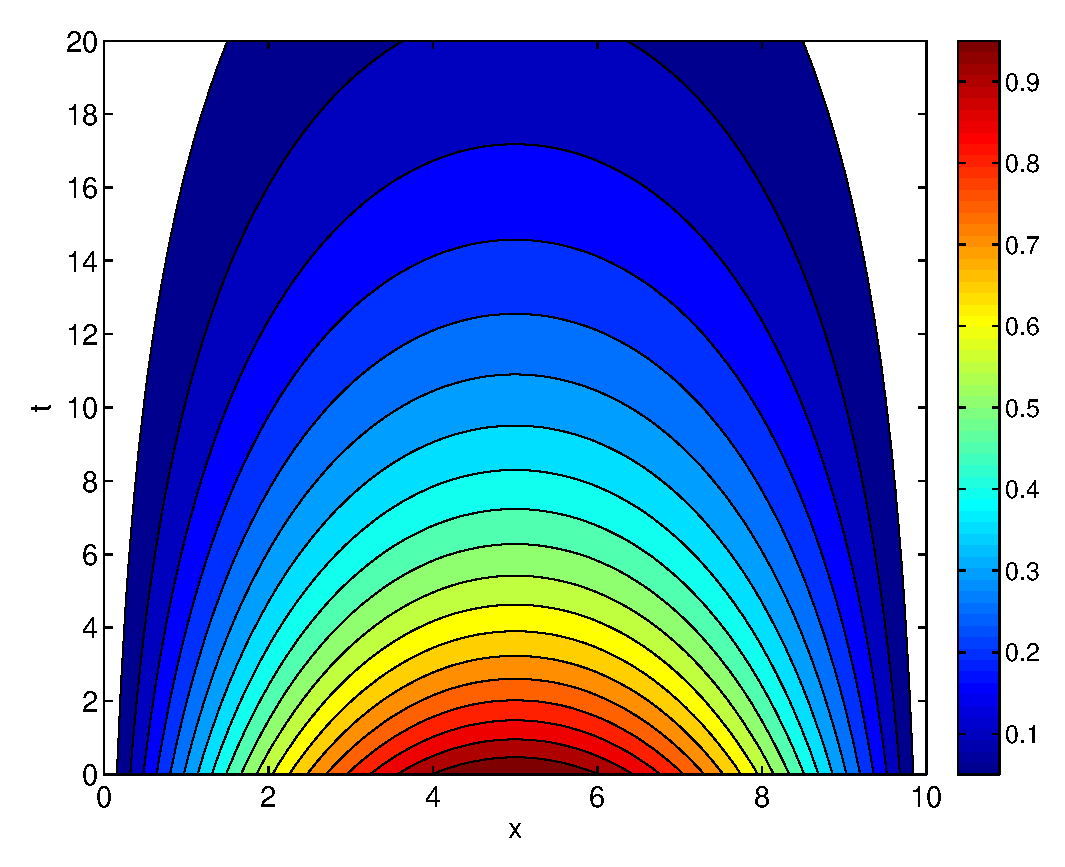
\includegraphics[scale=0.53]{checksol5}
      \end{center}

MATLAB code:
{\footnotesize \begin{verbatim}
 c = .385;
 kappa = 3.86;
 rho = 8.96;
 l = 10;
 theta = pi/l;

% first style: snapshots at t = 0, 4, 8, ..., 20
 t = 0:4:20;
 x = linspace(0,l,100);

 figure(1), clf
 for j=1:length(t)
    u = exp(-kappa*theta^2*t(j)/(rho*c))*sin(theta*x);  % compute u(:,t(j))
    plot(x,u,'k-','linewidth',2), hold on
    text(4.75, max(u)-.03, sprintf('t = %d', t(j)))
 end
 axis([0 10 0 1.1])
 set(gca,'fontsize',14)
 xlabel('x')
 ylabel('u(x,t)')
 print -depsc2 checksol1

% generate data for 3-d plots
 x = linspace(0,l,100);
 t = linspace(0,20,50);
 U = zeros(length(t), length(x));
 for j=1:length(t)
    U(j,:) = exp(-kappa*theta^2*t(j)/(rho*c))*sin(theta*x);
 end

% mesh plot
 figure(2), clf
 mesh(x,t,U,'edgecolor','k')
 view(-55,20)
 set(gca,'fontsize',14)
 xlabel('x'), ylabel('t'), zlabel('u(x,t)')
 print -depsc2 checksol2

% surf plot
 figure(3), clf
 surf(x,t,U)
 view(-55,20)
 set(gca,'fontsize',14)
 xlabel('x'), ylabel('t'), zlabel('u(x,t)')
 print -depsc2 checksol3

% waterfall plot
 figure(4), clf
 plt = waterfall(x,t,U);
 set(plt,'edgecolor','k')       % make the lines black
 view(-55,20)
 set(gca,'fontsize',14)
 xlabel('x'), ylabel('t'), zlabel('u(x,t)')
 print -depsc2 checksol4

% contour plot
 figure(5), clf
 [cs,h] = contourf(x,t,U,[.05:.05:.95],'k-');
 set(gca,'fontsize',14)
 xlabel('x'), ylabel('t')
 colorbar 
 print -depsc2 checksol5
\end{verbatim}}
\end{enumerate}
\end{solution}

